%%%%%%%%%%%%%%%%%%%%%%%%%%%%%%%%%%%%%%%%%
% Dreuw & Deselaer's Poster
% LaTeX Template
% Version 1.0 (11/04/13)
%
% Created by:
% Philippe Dreuw and Thomas Deselaers
% http://www-i6.informatik.rwth-aachen.de/~dreuw/latexbeamerposter.php
%
% This template has been downloaded from:
% http://www.LaTeXTemplates.com
%
% License:
% CC BY-NC-SA 3.0 (http://creativecommons.org/licenses/by-nc-sa/3.0/)
%
%%%%%%%%%%%%%%%%%%%%%%%%%%%%%%%%%%%%%%%%%

%----------------------------------------------------------------------------------

\documentclass[final,hyperref={pdfpagelabels=false}]{beamer}

\usepackage[orientation=portrait,size=a4,scale=1.4]{beamerposter} % Use the beamerposter package for laying out the poster with a portrait orientation and an a0 paper size

\usetheme{I6pd2} % Use the I6pd2 theme supplied with this template

\usepackage[czech,slovak,english]{babel}
\usepackage[utf8]{inputenc} %kodovani / encoding
\usepackage[T1]{fontenc}
\usepackage{listings}
\usepackage[figurename=]{caption}

\definecolor{LstColor}{HTML}{e3e2e0}

%\usepackage[english]{babel} % English language/hyphenation

\usepackage{amsmath,amsthm,amssymb,latexsym} % For including math equations, theorems, symbols, etc

\usepackage{times}\usefonttheme{professionalfonts}  % Uncomment to use Times as the main font
%\usefonttheme[onlymath]{serif} % Uncomment to use a Serif font within math environments

\boldmath % Use bold for everything within the math environment

\usepackage{booktabs} % Top and bottom rules for tables

\graphicspath{{figures/}} % Location of the graphics files

\usecaptiontemplate{\small\structure{\insertcaptionname~\insertcaptionnumber: }\insertcaption} % A fix for figure numbering

%----------------------------------------------------------------------------------

\title{\huge Komponentní systém pro herní grafický engine} % Poster title

\author{Tomáš Polášek} % Author(s)

\institute{Vysoké učení technické v Brně -- Fakulta informačních technologií} % Institution(s)

%----------------------------------------------------------------------------------

\newcommand{\leftfoot}{Entropy -- Entity-Component-System} % Left footer text

\newcommand{\rightfoot}{Tomáš Polášek} % Right footer text

%----------------------------------------------------------------------------------

\begin{document}

\addtobeamertemplate{block end}{}{\vspace*{2ex}} % White space under blocks

\begin{frame}[t, fragile] % The whole poster is enclosed in one beamer frame

\begin{columns}[t] % The whole poster consists of two major columns, each of which can be subdivided further with another \begin{columns} block - the [t] argument aligns each column's content to the top

\begin{column}{.02\textwidth}\end{column} % Empty spacer column

\begin{column}{.465\textwidth} % The first column

%----------------------------------------------------------------------------------

\begin{block}{Cíle}

\begin{itemize}
	\item Cílem byl návrh a implementace knihovny pro správu entit, která umožňuje vývoj pomocí \emph{Entity-Component-System} paradigmatu.
	\item Mezi požadavky patřily:
	\begin{enumerate}
		\item Možnosti paralelního provádění datových transformací.
		\item Efektivní použití vyrovnávacích pamětí.
		\item Intuitivní programovací rozhraní.
		\item Jednoduchá integrace do existujících projektů.
	\end{enumerate}
\end{itemize}


\end{block}

%----------------------------------------------------------------------------------

\begin{block}{Důvody}

\begin{itemize}
	\item Obvyklé návrhové prostředky -- jako \emph{objektově orientované programování} -- jsou pro návrh her příliš rigidní. 
	\item Zvyšující se požadavky na oddělení jednotlivých částí herního enginu.
	\item Výkonnostní rozdíl mezi přístupovou dobou pamětí a rychlostí vykonávání instrukcí se stále zvyšuje. 
	\item Vzniká \emph{datově orientovaný návrh}, jehož cílem je vyšší efektivita práce s fyzickým hardware -- vyrovnávací paměti, pipelining.
\end{itemize}

\end{block}

%----------------------------------------------------------------------------------

\begin{block}{Entity-Component-System}
	
	\begin{columns}
		\begin{column}{0.6\textwidth}
			\begin{itemize}
				\item Návrhové paradigma založené na kompozici. Vychází z principů \emph{datově orientovaného návrhu}.
			\end{itemize}
		\end{column}
		\begin{column}{0.29\textwidth}
			\hspace{-2em} 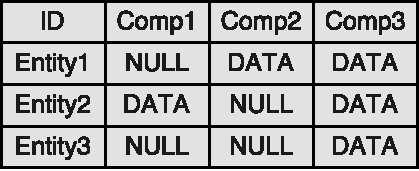
\includegraphics[width=1.2\linewidth]{BAC-POS0.pdf}
		\end{column}
	\end{columns}
	\begin{itemize}
		\item Striktní separace logiky a dat, čímž umožňuje vyšší úroveň modularity. 
		\item Skládá se ze tří částí -- \emph{entity}, \emph{komponenty} a \emph{systémy}.
	\end{itemize}

	
\end{block}

%----------------------------------------------------------------------------------

\begin{block}{Entity}
	
	\begin{itemize}
		\item \emph{Entity} reprezentují virtuální objekty uvnitř herního světa.
		\item Jejich hlavní funkcí je identifikace daného objektu a vazba na komponenty.
		\item Identifikátor \emph{entity} je primárním klíčem v tabulce \emph{entit}.
	\end{itemize}
	
\end{block}

%----------------------------------------------------------------------------------

\begin{block}{Komponenty}
	
	\begin{itemize}
		\item Základní nosiče dat a zároveň nejmenší datová jednotka, kterou lze \emph{entitám} přiřadit.
		\item Neobsahují \uv{výkonnou} logiku, pouze operace pro manipulaci dat.
		\item Sloupce tabulky \emph{entit} obsahují jednotlivé typy komponent.
	\end{itemize}
	
\end{block}

%----------------------------------------------------------------------------------

\begin{block}{Systémy}
	
	\begin{itemize}
		\item \emph{Systémy} implementují datové transformace nad \emph{entitami} a jejich \emph{komponentami}.
		\item Transformují pouze takové \emph{entity}, které obsahují požadované \emph{komponenty}.
	\end{itemize}
	
\end{block}

%----------------------------------------------------------------------------------

\end{column} % End of the first column

\begin{column}{.03\textwidth}\end{column} % Empty spacer column
 
\begin{column}{.465\textwidth} % The second column
	
%----------------------------------------------------------------------------------

\begin{block}{Výsledky}

\begin{itemize}
	\item Výsledkem je multiplatformní knihovna \textbf{Entropy}, která umožňuje návrh pomocí \emph{ECS} paradigmatu.
	\item Implementována v programovacím jazyce \emph{C++}.
\end{itemize}
\begin{columns}
	\begin{column}{0.6\linewidth}
		\vspace{-3em}
		\begin{itemize}
		\item Využívá koncept \emph{skupin}, které umožňují uchovávat seznamy filtrovaných \emph{entit}. \emph{Systémy} iterují pouze nad \emph{entitami}, které již skutečně obsahují požadované \emph{komponenty}.
		\end{itemize}
	\end{column}
	\begin{column}{0.29\linewidth}
		\vspace{-2em}
		\begin{figure}
			\hspace{-4em}
			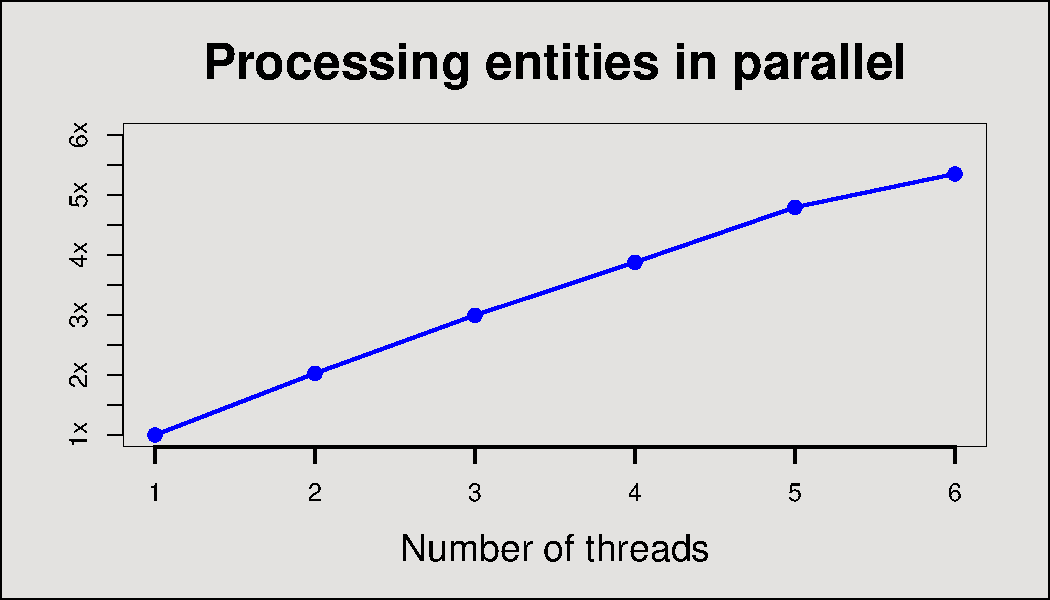
\includegraphics[scale=0.2]{poster0.pdf}
			\caption{\hspace{-6em} Lineární škálování s počtem vláken}
		\end{figure}
	\end{column}
\end{columns}
\vspace{-1em}
\begin{itemize}
	\item Umožňuje paralelizaci na třech úrovních:
	\begin{itemize}
		\item \emph{Entity} -- Rozdělení množiny \emph{entit} na jednotlivá vlákna, která provádí požadovanou transformaci odděleně.
		\item \emph{Systémy} -- Běh několika \emph{systémů} zároveň na rozdílných vláknech.
		\item \emph{Množiny změn} -- Pokud vlákna přistupují ke stejným zdrojům, je možné generovat \emph{množiny změn}. Tím je daná operace odložena na dobu, kdy ji bude možné vykonat bez synchronizace.
	\end{itemize}
\end{itemize}

\end{block}

%----------------------------------------------------------------------------------

\begin{block}{Použití}
	
	\begin{itemize}
		\item Knihovna \textbf{Entropy} je volně dostupná, pod licencí \emph{MIT}, z níže uvedeného repositáře projektu. 
		\item Příklad jednoduchého \emph{systému}, který implementuje pohyb \emph{entit}, definice \emph{komponenty}:
	\end{itemize}
	\begin{lstlisting}[backgroundcolor = \color{LstColor}, language = C++, xleftmargin = 0cm, framexleftmargin = 0em, tabsize=2]
	struct PositionC
	{
		float x, y;
		flot dX, dY;
	}
	\end{lstlisting}
	\begin{itemize}
		\item Definice \emph{systému}: 
	\end{itemize}
	\begin{lstlisting}[backgroundcolor = \color{LstColor}, language = C++, xleftmargin = 0cm, framexleftmargin = 0em, tabsize=2]
	struct MovementS : public System
	{
		using Require = Require<PositionC>;
		void doMove();
	}
	\end{lstlisting}
	\begin{itemize}
		\item Samotný posun entit: 
	\end{itemize}
	\begin{lstlisting}[backgroundcolor = \color{LstColor}, language = C++, xleftmargin = 0cm, framexleftmargin = 0em, tabsize=2]
	void doMove()
	{
		for (auto &e : foreach())
		{
			PositionC *p{e.get<PositionC>()};
			p->x += p->dX;
			p->y += p->dY;
		}
	}
	\end{lstlisting}
	
\end{block}

%----------------------------------------------------------------------------------

\setbeamercolor{block title}{fg=black,bg=orange!70} % Change the block title color

\vspace{1.2em}

\begin{block}{Kontaktní informace}
	
	\begin{itemize}
		\item GIT projektu: \href{https://github.com/T0mt0mp/Entropy}{https://github.com/T0mt0mp/Entropy}
		\item E-mail: \href{mailto:xpolas34@stud.fit.vutbr.cz}{xpolas34@stud.fit.vutbr.cz}
	\end{itemize}
	
\end{block}

%----------------------------------------------------------------------------------

\end{column} % End of the second column

\begin{column}{.015\textwidth}\end{column} % Empty spacer column

\end{columns} % End of all the columns in the poster

\end{frame} 

% End of the enclosing frame

\end{document}